\documentclass[11pt,a4paper]{article}
\usepackage[utf8]{inputenc}
\usepackage[T1]{fontenc}
\usepackage[margin=2.5cm]{geometry}
\usepackage{amsmath,amssymb,amsthm,mathtools}
\IfFileExists{lmodern.sty}{\usepackage{lmodern}}{}
\usepackage{graphicx,booktabs,enumitem}
\usepackage[expansion=false]{microtype}
\usepackage[dvipsnames]{xcolor}
\usepackage[most]{tcolorbox}
\usepackage[colorlinks=true,linkcolor=MidnightBlue,citecolor=MidnightBlue,urlcolor=MidnightBlue]{hyperref}
\usepackage{cleveref}

\graphicspath{{../figures/}}

\newtheorem{result}{Result}
\newtheorem{claim}{Claim}[section]
\theoremstyle{definition}
\newtheorem{exercise}{Exercise}[section]
\theoremstyle{remark}
\newtheorem*{remark}{Remark}

\newtcolorbox{intuition}{colback=Goldenrod!8,colframe=Goldenrod!70!black,
  title=Intuition,fonttitle=\bfseries\small,boxrule=0.5pt,arc=2pt}
\newtcolorbox{paperbox}[1]{colback=MidnightBlue!5,colframe=MidnightBlue!70,
  title={#1},fonttitle=\bfseries\small,boxrule=0.5pt,arc=2pt}
\newtcolorbox{warnbox}{colback=BrickRed!5,colframe=BrickRed!70,
  title=Check against the PDF,fonttitle=\bfseries\small,boxrule=0.5pt,arc=2pt}

\newcommand{\E}{\mathbb{E}}
\newcommand{\Prob}{\mathbb{P}}
\newcommand{\N}{\mathcal{N}}
\newcommand{\tA}{\tau_A}
\newcommand{\lI}{\lambda_I}
\newcommand{\lG}{\lambda_G}

\title{\textbf{AI, Human Cognition and Knowledge Collapse}\\[2pt]
\large A deep-immersion tutorial on Acemoglu, Kong \& Ozdaglar (2026)\\
\normalsize Part I --- the static problem, Observation 1, and the bridge to Lemma 2}
\author{Repository \texttt{ai-04-acemoglu} \textperiodcentered{} AI and Economic Modeling, UP 2026-II}
\date{Version read: author version dated 5 May 2026 of NBER Working Paper 34910 (69 pp.)}

\begin{document}
\maketitle

\begin{abstract}
\noindent This tutorial rebuilds, step by step, the part of the paper the course asks us to master: the
environment, the Bayesian updating that turns effort into \emph{precision}, the agent's static problem, and
\textbf{Observation 1} --- the two cross-partial signs on which the whole paper rests. It then crosses the
bridge to the dynamics just far enough to see \emph{why} the Frisch elasticity threshold $\varepsilon=4$ in
Lemma~2 appears. Nothing is taken on trust: every step says which rule it uses. Proofs of the
dynamic and welfare results (Propositions 3--14) are read, not reproduced.
\end{abstract}

\begin{warnbox}
The paper circulates in two versions: the NBER working paper (February 2026) and the MIT author
version dated \textbf{5 May 2026}, which is the one the course repository distributes. \textbf{We read and
cite the 5 May 2026 version}; page numbers are its printed pages. The model is \S3 (\S2 is the related
literature), Observation~1 is in \S3.4 (p.~14) and Observation~2 in \S3.5 (p.~16). The February version
writes the effort cost as $\frac1\alpha e^\alpha$ and every threshold as $\alpha-1\gtrless\frac14$; it is the
same model under $\varepsilon=1/(\alpha-1)$. A sentence-by-sentence comparison of the two versions is in
\texttt{extra/version-comparison.md}.
\end{warnbox}

\tableofcontents

%======================================================================
\section{The question in one paragraph}
%======================================================================

A doctor needs two kinds of knowledge to treat a patient: \emph{general} knowledge (how the disease works)
and \emph{context-specific} knowledge (what this patient has). General knowledge is a public good produced
by many people's learning and it depreciates as the world changes; context-specific knowledge is private
and useless next period. Agentic AI --- a system that gives each person a tailored recommendation ---
supplies context-specific knowledge. The paper asks:
\begin{quote}
\emph{If AI makes it cheaper to know the specific answer, do people stop investing in the general
understanding that everyone else also relies on --- and can society's stock of general knowledge
collapse as a result?}
\end{quote}
The answer rests on two signs: general knowledge \emph{complements} human effort, agentic AI
\emph{substitutes} for it. Everything dynamic in the paper is the consequence of feeding those two signs
into a precision recursion.

\begin{intuition}
Week 1 (Aouad--Lykouris--Zhong) had skill, effort and AI enter production as a sum, $x=s+e+a$, pushed
through a concave $p(\cdot)$. Here the same thing happens one level down: human learning and AI enter as a
sum of \emph{precisions}, $Y=\sigma^{-2}+\lI e+\tA$, pushed through a concave accuracy function $G(\cdot)$.
The substitution half of Observation 1 is ALZ's mechanism in Bayesian clothing. What is new is the other
half --- the complementarity with a public stock $X$ that itself evolves.
\end{intuition}

%======================================================================
\section{The environment (\S3.1)}
%======================================================================

\subsection{Two states of the world}
Time is discrete, $t=1,2,\dots$. There is a continuum of agents $i$, grouped in ``islands'' $m$ of mass
$I$ (the \emph{aggregation capacity}).
\begin{align}
\text{common state (general knowledge):}\quad & \theta_{t+1}=\theta_t+\varepsilon_t,\quad
\varepsilon_t\sim\N(0,\Sigma^2),\quad \theta_1\sim\N(0,\Sigma_0^2), \label{eq:common}\\
\text{idiosyncratic state (context):}\quad & \theta_{i,t}\overset{\text{iid}}{\sim}\N(0,\sigma^2).
\label{eq:idio}
\end{align}
Two features matter for everything that follows:
\begin{itemize}[nosep]
\item $\theta_t$ is a \textbf{random walk}: yesterday's general knowledge is still useful today, but it
\emph{depreciates} because the truth keeps moving (variance $\Sigma^2$ added every period).
\item $\theta_{i,t}$ is \textbf{iid over time}: context knowledge has no future value at all.
\end{itemize}

\subsection{Task, production and the three $\Delta$'s}
Each period agent $i$ predicts $\theta_t$ with $x_{i,t}$ and $\theta_{i,t}$ with $y_{i,t}$. A prediction is
``good'' if it is within distance $1$ of the truth. Output is
\[
f\bigl(\mathbf 1\{|x_{i,t}-\theta_t|\le 1\},\;\mathbf 1\{|y_{i,t}-\theta_{i,t}|\le 1\}\bigr),
\]
with $f:\{0,1\}^2\to\mathbb R$ weakly increasing and normalised so that $f(1,1)-f(0,0)=1$.
Define
\[
\Delta_G:=f(1,0)-f(0,0),\qquad \Delta_I:=f(0,1)-f(0,0),\qquad \Delta_X:=f(1,1)-f(1,0)-f(0,1)+f(0,0),
\]
so that $\Delta_G+\Delta_I+\Delta_X=1$. $\Delta_X$ is a discrete cross-partial: it measures how much getting
\emph{both} right is worth beyond getting each right separately.

\begin{claim}[Multilinear form of $f$]\label{cl:multilinear}
For all $(a,b)\in\{0,1\}^2$: \quad $f(a,b)=f(0,0)+\Delta_G\,a+\Delta_I\,b+\Delta_X\,ab.$
\end{claim}
\begin{proof}
Check the four points. $(0,0)$: trivial. $(1,0)$: $f(0,0)+\Delta_G=f(1,0)$ by definition of $\Delta_G$.
$(0,1)$: likewise with $\Delta_I$. $(1,1)$: $f(0,0)+\Delta_G+\Delta_I+\Delta_X=f(1,1)$ by definition of
$\Delta_X$ (the $f(1,0)$ and $f(0,1)$ terms cancel).
\end{proof}

\begin{paperbox}{Assumption 1 (Complementarity)}
\[\Delta_I=0\qquad\text{and}\qquad \Delta_X>0.\]
The authors' justification (p.~9): context-specific knowledge alone, without general
knowledge, creates no value --- ``a doctor who observes a patient's symptoms may still be unable to provide
effective treatment without a correct understanding of the disease mechanisms.'' They call it ``a strong
complementarity between general and context-specific knowledge''; $\Delta_G>0$ is allowed; the Leontief $f(x,y)=\min\{x,y\}$ is the
canonical example ($\Delta_I=\Delta_G=0$, $\Delta_X=1$).
\end{paperbox}

\noindent Keep an eye on $\Delta_I=0$. It is a statement about \emph{production}, it is imposed from the
start, and --- as Part II will show --- it is never relaxed in Section~5. It is harmless for Observation 1
(\cref{rem:DI}) but it is not harmless for the collapse state or for the welfare limit.

\subsection{Effort, signals and AI}
Effort $e_{i,t}\ge0$ costs $\frac{\varepsilon}{\varepsilon+1}e_{i,t}^{(\varepsilon+1)/\varepsilon}$ (p.~9), so
marginal cost is $e^{1/\varepsilon}$ and $\varepsilon>0$ is the constant \textbf{Frisch elasticity} of effort
supply: if marginal benefit is $b$, effort is $b^{\varepsilon}$, so $\partial\ln e/\partial\ln b=\varepsilon$.
(February dictionary: $\frac1\alpha e^\alpha$ with $\alpha=1+1/\varepsilon$, so $\alpha-1>\frac14\iff\varepsilon<4$.)
Effort buys two signals:
\begin{align}
\text{private:}\quad & s^H_{i,t}\sim\N\bigl(\theta_{i,t},\,(\lI e_{i,t})^{-1}\bigr),\\
\text{public (island-level):}\quad & s^C_{m,t}\sim\N\bigl(\theta_t,\,(\lG E_{m,t})^{-1}\bigr),\qquad
E_{m,t}=\textstyle\int_{i\in m}e_{i,t}\,di,
\end{align}
and, after AI arrives, each agent also receives
\begin{equation}
\text{agentic AI:}\quad s^A_{i,t}\sim\N\bigl(\theta_{i,t},\,\tA^{-1}\bigr),\qquad \tA\ge0
\text{ (AI accuracy).}
\end{equation}
\textbf{Read this carefully:} the AI signal is about the \emph{idiosyncratic} state. Agentic AI in this model
gives you the answer for your case; it does not produce general knowledge. One person's effort is a
\emph{joint product}: it teaches her about her own case and, pooled with her island, about the common state.

%======================================================================
\section{Bayesian updating in precisions (\S3.2)}
%======================================================================

\subsection{The one Normal--Normal fact we need}
\begin{claim}\label{cl:nn}
If $\theta\sim\N(\mu,\tau_0^{-1})$ and, given $\theta$, $s\sim\N(\theta,\tau_s^{-1})$, then
$\theta\mid s\sim\N\!\left(\frac{\tau_0\mu+\tau_s s}{\tau_0+\tau_s},\,(\tau_0+\tau_s)^{-1}\right)$:
\textbf{precisions add}.
\end{claim}
\begin{proof}
By Bayes, the posterior density is proportional to
$\exp\{-\tfrac{\tau_0}{2}(\theta-\mu)^2-\tfrac{\tau_s}{2}(s-\theta)^2\}$. The exponent is a quadratic in
$\theta$ with coefficient $-\tfrac12(\tau_0+\tau_s)$ on $\theta^2$ and $(\tau_0\mu+\tau_s s)$ on $\theta$.
Completing the square gives $-\frac{\tau_0+\tau_s}{2}\bigl(\theta-\frac{\tau_0\mu+\tau_s s}{\tau_0+\tau_s}\bigr)^2$
plus terms free of $\theta$, which is the kernel of the stated Normal.
\end{proof}
Independent signals therefore just stack. This is why the whole paper can be written in precisions.

\subsection{Idiosyncratic precision}
For $\theta_{i,t}$ the agent has the prior ($\sigma^{-2}$), her own signal ($\lI e_{i,t}$) and the AI
($\tA$). By \cref{cl:nn} applied twice,
\begin{equation}\label{eq:Y}
Y_{i,t}=\sigma^{-2}+\lI e_{i,t}+\tA. \tag{4}
\end{equation}
Human learning and AI are \textbf{perfect substitutes in precision}. Nothing else in the model makes them
substitutes; the rest comes from curvature.

\subsection{Public precision and the Kalman recursion}
Let $X_t:=V_t^{-1}$ with $V_t=\mathrm{Var}(\theta_t\mid\mathcal I_t)$ the variance of the common state given
public information at the start of $t$. During $t$ the island's public signal arrives with precision
$\lG E_t$, so by \cref{cl:nn} the precision about $\theta_t$ becomes $X_t+\lG E_t$, i.e.\ variance
$(X_t+\lG E_t)^{-1}$. Then the state moves, $\theta_{t+1}=\theta_t+\varepsilon_t$, and independent variances
add:
\begin{equation}\label{eq:kalman}
X_{t+1}^{-1}=(X_t+\lG E_t)^{-1}+\Sigma^2. \tag{3}
\end{equation}
Two limits to internalise: with no learning ($E_t=0$), $X_{t+1}=X_t/(1+\Sigma^2X_t)<X_t$ --- knowledge
\textbf{depreciates}; and no amount of learning can push $X_{t+1}$ above $\Sigma^{-2}$, because tomorrow's
shock is unknowable today.

\subsection{From precision to accuracy: the function $G$}
With Bayesian predictions (posterior means), the prediction error given information is $\N(0,\tau^{-1})$,
where $\tau$ is the relevant posterior precision. The probability of being within $1$ is
\begin{equation}\label{eq:G}
G(\tau):=\Prob(|Z|\le1),\quad Z\sim\N(0,\tau^{-1})
\qquad\Longrightarrow\qquad
G(\tau)=\Prob\bigl(|W|\le\sqrt\tau\bigr)=2\Phi(\sqrt\tau)-1,
\end{equation}
where $W=\sqrt\tau\,Z\sim\N(0,1)$.

\begin{claim}[Everything we need about $G$]\label{cl:G}
On $\tau>0$:
\begin{enumerate}[label=(\alph*),nosep]
\item $g(\tau):=G'(\tau)=\dfrac{\phi(\sqrt\tau)}{\sqrt\tau}=\dfrac{1}{\sqrt{2\pi}}\,\tau^{-1/2}e^{-\tau/2}>0$;
\item $g'(\tau)=-\,g(\tau)\,\dfrac{1+\tau}{2\tau}<0$, so $G$ is strictly concave;
\item $G(0)=0$, $G(\infty)=1$, and $G(\tau)=\sqrt{2\tau/\pi}\,\bigl(1+O(\tau)\bigr)$ as $\tau\downarrow0$.
\end{enumerate}
\end{claim}
\begin{proof}
(a) Chain rule: $\frac{d}{d\tau}2\Phi(\sqrt\tau)=2\phi(\sqrt\tau)\cdot\frac{1}{2\sqrt\tau}$, and
$\phi(\sqrt\tau)=(2\pi)^{-1/2}e^{-\tau/2}$.
(b) Product rule on $(2\pi)^{-1/2}\tau^{-1/2}e^{-\tau/2}$:
$(2\pi)^{-1/2}e^{-\tau/2}\bigl(-\tfrac12\tau^{-3/2}-\tfrac12\tau^{-1/2}\bigr)
=-(2\pi)^{-1/2}\tau^{-1/2}e^{-\tau/2}\cdot\frac{1+\tau}{2\tau}$.
(c) $\Phi(0)=\tfrac12$ gives $G(0)=0$; $\Phi(\infty)=1$ gives $G(\infty)=1$. A first-order Taylor expansion
$\Phi(u)=\tfrac12+\phi(0)u+O(u^3)$ with $u=\sqrt\tau$ gives $G(\tau)=2\phi(0)\sqrt\tau+O(\tau^{3/2})$ and
$2\phi(0)=\sqrt{2/\pi}$.
\end{proof}

\begin{figure}[h]
\centering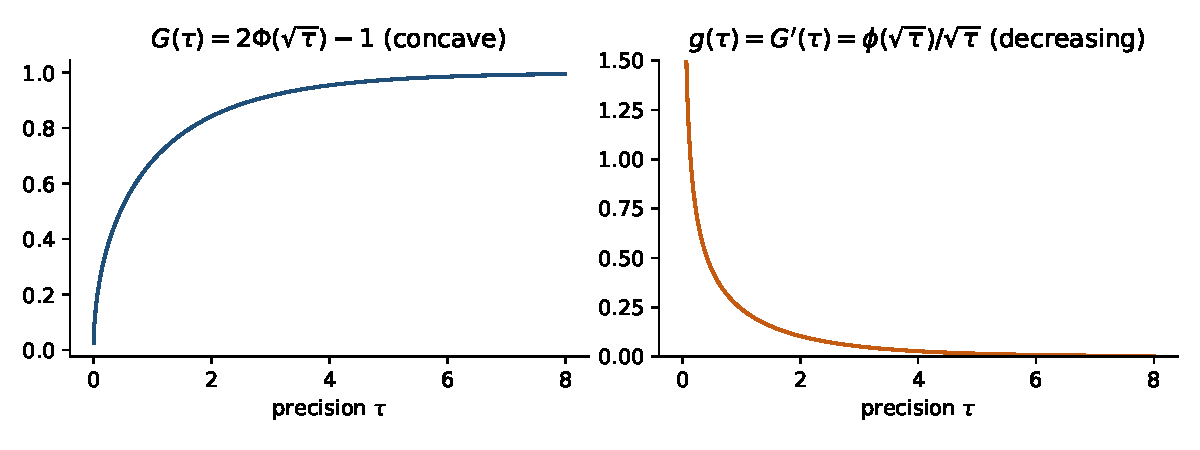
\includegraphics[width=0.85\textwidth]{fig1_G_g.pdf}
\caption{Accuracy is concave in precision: each extra unit of precision buys less accuracy. Note also the
square-root behaviour at $0$: $g(\tau)\to\infty$ as $\tau\downarrow0$.}
\end{figure}

\begin{intuition}
(b) is the engine of substitution: the more precise you already are about your case (because the AI told
you), the less an extra unit of your own learning improves the chance of getting it right. (c) is the engine
of collapse: when general knowledge is scarce, its value grows only like $\sqrt X$, so incentives to learn
vanish \emph{faster} than linearly as $X\to0$.
\end{intuition}

%======================================================================
\section{Expected payoff (equation 6)}
%======================================================================

Let $A=\{|x_{i,t}-\theta_t|\le1\}$ and $B=\{|y_{i,t}-\theta_{i,t}|\le1\}$. Given information,
$\Prob(A)=G(X_t)$ and $\Prob(B)=G(Y_{i,t})$. The two errors are independent: they are built from independent
states with independent priors and independent signals. Hence $\Prob(A\cap B)=G(X_t)G(Y_{i,t})$, and taking
expectations in \cref{cl:multilinear}:
\begin{equation}\label{eq:U}
U_{i,t}=f(0,0)+\Delta_G\,G(X_t)+\Delta_I\,G(Y_{i,t})+\Delta_X\,G(X_t)\,G(Y_{i,t})
-\tfrac{\varepsilon}{\varepsilon+1}e_{i,t}^{(\varepsilon+1)/\varepsilon}.
\end{equation}
Under Assumption 1 the $\Delta_I$ term drops and we get the paper's equation (6).

\begin{remark}[Timing]
The general-knowledge accuracy at $t$ is $G(X_t)$, i.e.\ it uses public information \emph{before} this
period's public signal. So period-$t$ effort improves general knowledge only from $t+1$ on. That is what
makes the problem below static.
\end{remark}

%======================================================================
\section{The agent's problem}
%======================================================================

\subsection{Why the problem is static}
Agent $i$ is atomistic: her own effort does not change $E_{m,t}$ and therefore does not change
$X_{t+1}$. Her private signal only teaches her about $\theta_{i,t}$, which is iid and worthless tomorrow.
So \emph{even a forward-looking agent} maximises \eqref{eq:U} period by period. The static problem is not
an assumption of myopia; it is the consequence of general knowledge being a public good. The flip side is
the \textbf{externality}: nobody is paid for the contribution of her effort to $X_{t+1}$.

\subsection{Statement}
Dropping terms that do not depend on $e$, and imposing Assumption 1,
\begin{equation}\label{eq:problem}
e(X,\tA)=\arg\max_{e\ge0}\ \Pi(e;X,\tA):=\Delta_X\,G(X)\,G(\sigma^{-2}+\lI e+\tA)-
\frac{\varepsilon}{\varepsilon+1}e^{\frac{\varepsilon+1}{\varepsilon}}.
\end{equation}

\begin{claim}[Existence, uniqueness, interiority]\label{cl:br}
Assume $\sigma^{-2}>0$. If $X>0$, \eqref{eq:problem} has a unique solution, it is interior, and it is the
unique root of the first-order condition
\begin{equation}\label{eq:foc}
\boxed{\;\Delta_X\,G(X)\,\lI\,g\bigl(\sigma^{-2}+\lI e+\tA\bigr)=e^{1/\varepsilon}\;}
\end{equation}
If $X=0$, then $e(0,\tA)=0$.
\end{claim}
\begin{proof}
$\Pi_e(e)=\Delta_XG(X)\lI g(Y)-e^{1/\varepsilon}$ and, for $e>0$,
$\Pi_{ee}(e)=\Delta_XG(X)\lI^2g'(Y)-\tfrac1\varepsilon e^{1/\varepsilon-1}<0$, using $g'<0$ from
\cref{cl:G}(b). So $\Pi_e$ is strictly decreasing. At $e=0$: $\Pi_e(0)=\Delta_XG(X)\lI g(\sigma^{-2}+\tA)$,
finite because $\sigma^{-2}+\tA>0$, and strictly positive iff $X>0$ (as $G(X)>0\iff X>0$). As $e\to\infty$,
$g(Y)\to0$ while $e^{1/\varepsilon}\to\infty$, so $\Pi_e\to-\infty$. By continuity and strict monotonicity,
$\Pi_e$ has exactly one root $e^*>0$ when $X>0$, and $\Pi$ is strictly concave, so the root is the global
maximiser on $[0,\infty)$. When $X=0$, $\Pi_e(e)=-e^{1/\varepsilon}<0$ for all $e>0$, so $e^*=0$.
\end{proof}

\begin{intuition}
Marginal cost of effort is zero at $e=0$ (because the cost exponent $(\varepsilon+1)/\varepsilon>1$), so any
positive marginal benefit gets a positive response: no corner unless the benefit is exactly zero.
Contrast with week 1, where linear cost made the corner $e=0$ the main story. Here the corner happens only
at $X=0$ --- and that is precisely the collapse state.
\end{intuition}

%======================================================================
\section{Observation 1: the two cross-partials (\S3.4)}
%======================================================================

\begin{paperbox}{Observation 1 (\S3.4, p.~14)}
Under Assumption 1, for $X_t>0$:
\[
\frac{\partial^2U_{i,t}}{\partial e_{i,t}\,\partial X_t}>0,\qquad
\frac{\partial^2U_{i,t}}{\partial e_{i,t}\,\partial\tA}<0.
\]
General knowledge complements human effort; agentic AI substitutes for it.
\end{paperbox}

\begin{proof}[Derivation]
Differentiate \eqref{eq:U} with $\Delta_I=0$ once in $e$:
\[
U_e=\Delta_X\,G(X)\,\lI\,g(Y)-e^{1/\varepsilon},\qquad Y=\sigma^{-2}+\lI e+\tA .
\]
\emph{Complementarity.} The cost term does not depend on $X$; $Y$ does not depend on $X$. Product rule on
$G(X)$:
\[
U_{eX}=\Delta_X\,\lI\,\underbrace{g(X)}_{>0}\,\underbrace{g(Y)}_{>0}>0 .
\]
\emph{Substitution.} The cost term does not depend on $\tA$; $\partial Y/\partial\tA=1$. Chain rule on
$g(Y)$:
\[
U_{e\tA}=\Delta_X\,G(X)\,\lI\,\underbrace{g'(Y)}_{<0}<0\qquad(X>0).
\]
\end{proof}

\noindent Notice what each sign uses --- this is the kind of bookkeeping the oral exam rewards:
\begin{center}
\begin{tabular}{@{}lll@{}}
\toprule
Sign & What delivers it & Where the assumption lives\\
\midrule
$U_{eX}>0$ & $\Delta_X>0$ and $g>0$ & production side ($f$ is supermodular)\\
$U_{e\tA}<0$ & $g'<0$ ($G$ concave) and $Y$ additive & information side (Gaussian precisions)\\
\bottomrule
\end{tabular}
\end{center}

\begin{remark}[What if $\Delta_I>0$?]\label{rem:DI}
With the $\Delta_I$ term in \eqref{eq:U}, $U_e=\lI\,g(Y)\,[\Delta_I+\Delta_XG(X)]-e^{1/\varepsilon}$. Then
$U_{eX}=\lI g(Y)\Delta_Xg(X)>0$ and $U_{e\tA}=\lI g'(Y)[\Delta_I+\Delta_XG(X)]<0$: \textbf{Observation 1
survives}, and now even at $X=0$. What changes is \cref{cl:br}: at $X=0$ the marginal benefit is
$\lI\Delta_Ig(\sigma^{-2}+\tA)>0$, so $e(0,\tA)>0$. Part II builds on this.
\end{remark}

%======================================================================
\section{Observation 2: monotone best response}
%======================================================================

\begin{paperbox}{Observation 2 (\S3.5, p.~16)}
$e(X,\tA)$ is increasing in $X$ and decreasing in $\tA$, strictly so for all $X>0$.
\end{paperbox}

\subsection{Route 1: implicit function theorem}
For $X>0$ the best response is the interior root of $\Pi_e(e;X,\tA)=0$ with $\Pi_{ee}<0$, so the IFT applies:
\begin{align}
\frac{\partial e}{\partial X}&=-\frac{\Pi_{eX}}{\Pi_{ee}}
=\frac{\Delta_X\lI\,g(X)\,g(Y)}{\tfrac1\varepsilon e^{1/\varepsilon-1}+\Delta_XG(X)\lI^2|g'(Y)|}>0,\\[4pt]
\frac{\partial e}{\partial \tA}&=-\frac{\Pi_{e\tA}}{\Pi_{ee}}
=-\frac{\Delta_XG(X)\lI\,|g'(Y)|}{\tfrac1\varepsilon e^{1/\varepsilon-1}+\Delta_XG(X)\lI^2|g'(Y)|}<0.
\label{eq:detau}
\end{align}

\subsection{Route 2: Topkis}
$\Pi$ has strictly increasing differences in $(e,X)$ and strictly decreasing differences in $(e,\tA)$
(Observation 1), and $\arg\max$ is a singleton. Topkis' monotonicity theorem gives the same conclusion
\emph{without} differentiability of the solution. This is the route the paper cites (p.~16).

\subsection{A result the paper does not state: crowding-out is partial}
\begin{result}\label{res:partial}
At a fixed $X>0$, $\displaystyle \frac{dY}{d\tA}=1+\lI\frac{\partial e}{\partial\tA}\in(0,1)$.
AI crowds out human learning, but less than one-for-one: holding general knowledge fixed, total
idiosyncratic precision rises with AI accuracy.
\end{result}
\begin{proof}
From \eqref{eq:detau}, with $a:=\tfrac1\varepsilon e^{1/\varepsilon-1}>0$ and $b:=\Delta_XG(X)\lI^2|g'(Y)|>0$,
$\lI\,\partial e/\partial\tA=-b/(a+b)\in(-1,0)$.
\end{proof}
\noindent This is why, in Proposition~4, $\bar Y_h$ is increasing in $\tA$ when $\varepsilon<4$; and why the
\emph{non}-monotonicity of $\bar Y_h$ in Proposition~8 ($\varepsilon>4$) must come from the fall in $X$, not
from the static problem.

\subsection{Effort near $X=0$}
\begin{result}\label{res:small}
As $X\downarrow0$, \ $e(X,\tA)=\kappa(\tA)\,X^{\varepsilon/2}\,(1+o(1))$, with
$\kappa(\tA):=\bigl(\sqrt{2/\pi}\;\Delta_X\lI\,g(\sigma^{-2}+\tA)\bigr)^{\varepsilon}$, decreasing in $\tA$.
\end{result}
\begin{proof}
Raise \eqref{eq:foc} to the power $\varepsilon$: $e=\bigl(\Delta_X\lI G(X)g(Y)\bigr)^\varepsilon$. As
$X\downarrow0$, $e\to0$ (by Observation 2 and $e(0,\tA)=0$), so $g(Y)\to g(\sigma^{-2}+\tA)$ by continuity; and
$G(X)=\sqrt{2X/\pi}\,(1+O(X))$ by \cref{cl:G}(c). Multiply.
\end{proof}

%======================================================================
\section{The bridge to the dynamics (read-only, but understood)}
%======================================================================

\subsection{Equilibrium in one line}
In a symmetric equilibrium $E_t=Ie_t$ and $e_t=e(X_t,\tA)$. Plugging into \eqref{eq:kalman}
(Proposition~1):
\[
X_{t+1}=F(X_t):=\Bigl[\Sigma^2+\bigl(X_t+\lG I\,e(X_t,\tA)\bigr)^{-1}\Bigr]^{-1}.
\]
$F$ is continuous and strictly increasing, $F(0)=0$, $F(\infty)=\Sigma^{-2}$ (Lemma~1). Since $F$ is
increasing, the orbit $X_t$ is monotone, and it converges to a fixed point: the whole dynamics is read off
the 45-degree diagram.

\subsection{The maintenance-effort curve}
\begin{claim}\label{cl:maint}
For $0<X<\Sigma^{-2}$,
\[
F(X)>X\iff e(X,\tA)>e_m(X):=\frac{\Sigma^2X^2}{\lG I\,(1-\Sigma^2X)} ,
\]
and $F(X)<X$ for every $X\ge\Sigma^{-2}$. Positive steady states are the intersections of $e(\cdot,\tA)$
with $e_m(\cdot)$.
\end{claim}
\begin{proof}
Let $z=X+\lG Ie$. $F(X)>X\iff \Sigma^2+z^{-1}<X^{-1}\iff z^{-1}<\frac{1-\Sigma^2X}{X}$. If
$1-\Sigma^2X>0$ both sides are positive, so invert: $z>\frac{X}{1-\Sigma^2X}$, i.e.
$\lG Ie>\frac{X}{1-\Sigma^2X}-X=\frac{\Sigma^2X^2}{1-\Sigma^2X}$. If $X\ge\Sigma^{-2}$ the right side is
$\le0<z^{-1}$, so $F(X)<X$.
\end{proof}
\noindent $e_m(X)$ is the effort needed to exactly offset one period of depreciation. It separates the two
comparative statics cleanly: $\tA$ shifts the \emph{effort} curve down (Observation 2); $I$ shifts the
\emph{maintenance} curve down ($e_m\propto1/I$). That is Proposition~2 in one picture.

\subsection{Why $\varepsilon=4$: Lemma 2 by comparing exponents}
Near $0$, $e_m(X)=\frac{\Sigma^2}{\lG I}X^2(1+O(X))$ and, by \cref{res:small},
$e(X,\tA)=\kappa X^{\varepsilon/2}(1+o(1))$.
\begin{itemize}[nosep]
\item $\varepsilon<4$: $\varepsilon/2<2$, so $e>e_m$ for all small $X>0$, hence $F(X)>X$: a small stock of
knowledge \emph{grows}; $X=0$ is locally unstable.
\item $\varepsilon>4$: $\varepsilon/2>2$, so $e<e_m$ for small $X$, hence $F(X)<X$: the orbit decreases,
stays positive, and converges to $0$; $X=0$ is locally stable --- a \textbf{knowledge-collapse trap}.
\item $\varepsilon=4$: both are $\propto X^2$ and the answer depends on $\kappa(\tA)$ versus
$\Sigma^2/(\lG I)$ --- a knife edge.
\end{itemize}

\begin{figure}[h]
\centering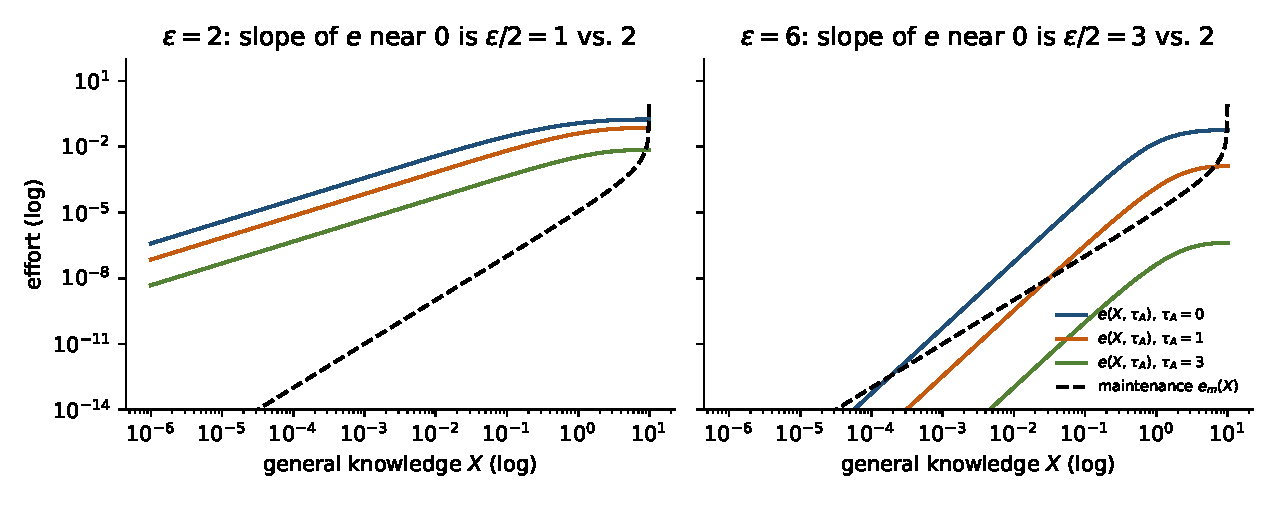
\includegraphics[width=\textwidth]{fig2_effort_vs_maintenance.pdf}
\caption{Log--log plot of best-response effort $e(X,\tA)$ (solid) and maintenance effort $e_m(X)$
(dashed). Near $0$ the slopes are $\varepsilon/2$ and $2$. Left ($\varepsilon=2$): effort always
eventually exceeds maintenance, one positive steady state. Right ($\varepsilon=6$): effort starts below
maintenance, so there is a low unstable crossing $\bar X_m$ and a high stable one $\bar X_h$ --- until AI is
accurate enough ($\tA=3$) that the curves never cross and collapse is global. Parameters in
\texttt{sim/model.py}.}
\label{fig:loglog}
\end{figure}

\begin{remark}[Why the linearisation is useless]
$F(X)=z/(1+\Sigma^2z)$ with $z=X+\lG Ie(X)$. For $\varepsilon>2$, $e'(0)=0$, so $F'(0)=1$: the collapse
steady state is \emph{non-hyperbolic} and its stability is decided by second-order terms. That is why the
threshold is a comparison of exponents ($\varepsilon/2$ versus $2$) and not an eigenvalue condition.
Numerically it also means convergence to $0$ is slow ($X_t\approx1/(\Sigma^2t)$): a collapse is a drift,
not a crash.
\end{remark}

\begin{intuition}
Depreciation of \emph{precision} is quadratic: a random-walk shock removes about $\Sigma^2X^2$ of precision
per period when $X$ is small. The incentive to learn when general knowledge is scarce is $\propto G(X)\approx
\sqrt X$, and effort responds with elasticity $\varepsilon$, so effort $\propto X^{\varepsilon/2}$. Collapse
is self-reinforcing exactly when people are responsive enough ($\varepsilon>4$) that effort vanishes faster
than the maintenance requirement.
\end{intuition}

\begin{figure}[h]
\centering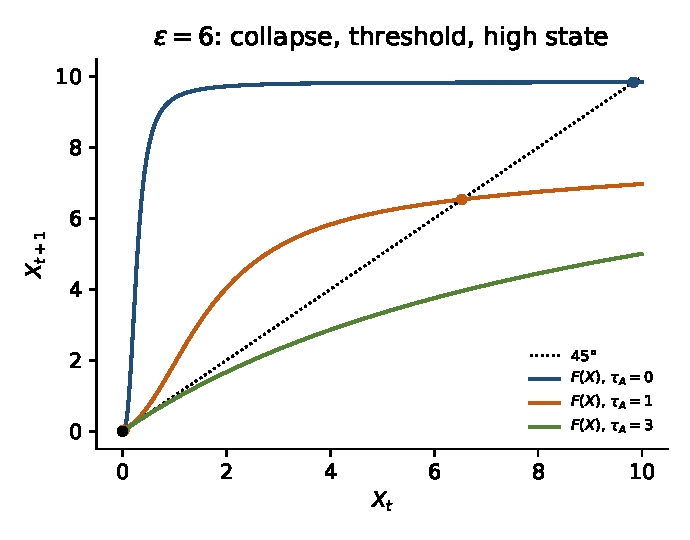
\includegraphics[width=0.55\textwidth]{fig3_45degree_eps6.pdf}
\caption{The 45-degree diagram for $\varepsilon=6$. For $\tA\in\{0,1\}$ there are two positive fixed points
(the lower one, $\bar X_m$, is very close to $0$ at these parameters; see \cref{fig:loglog}); at $\tA=3$ the
map lies below the diagonal everywhere and every orbit collapses.}
\end{figure}

\subsection{The dynamic results at a glance (read, do not reproduce)}
\begin{center}\small
\begin{tabular}{@{}p{2.2cm}p{11.8cm}@{}}
\toprule
Result & Content\\
\midrule
Prop.~3 ($\varepsilon<4$) & Steady states $0=\bar X_\ell<\bar X_h$; $\bar X_h$ globally stable from any $X_1>0$.\\
Prop.~4 ($\varepsilon<4$) & $\bar X_h,\bar e_h\downarrow$ and $\bar Y_h\uparrow$ in $\tA$; all $\uparrow$ in $I$.\\
Prop.~5 ($\varepsilon>4$) & Threshold $\tA^c$: below it, $0<\bar X_m<\bar X_h$ with basins split at $\bar X_m$; at or above it, collapse from every $X_1$.\\
Prop.~6 & $\tA^c$ increasing in $I$ and in $\Delta_X$.\\
Prop.~7 & $\bar X_m$ increasing in $\tA$, decreasing in $I$ and $\Delta_X$ (the trap widens with AI).\\
Prop.~8 ($\varepsilon>4$) & $\bar X_h,\bar e_h\downarrow$ in $\tA$; $\bar Y_h$ first up, then down.\\
\bottomrule
\end{tabular}
\end{center}
Every entry is one of two curves in \cref{fig:loglog} moving: $\tA$ pushes effort down, $I$ pushes
maintenance down, $\Delta_X$ scales effort up.

%======================================================================
\section{The main result with all its conditions}
%======================================================================

\begin{center}
\begin{tabular}{@{}p{4.2cm}p{10cm}@{}}
\toprule
Condition & Role\\
\midrule
Gaussian states and signals & Precisions add (\cref{cl:nn}); $G(\tau)=2\Phi(\sqrt\tau)-1$ is concave\\
Additive precision $Y=\sigma^{-2}+\lI e+\tA$ & AI and learning are perfect substitutes in precision\\
Assumption 1: $\Delta_I=0$, $\Delta_X>0$ & Complementarity sign; $e(0,\tA)=0$ so $X=0$ is a steady state\\
$\sigma^{-2}>0$ & Marginal benefit finite at $e=0$ even with $\tA=0$\\
Isoelastic cost, $\varepsilon>0$ & Interior best response; $\varepsilon$ vs.\ $4$ splits the regimes\\
Atomistic agents, iid $\theta_{i,t}$ & Static problem; learning externality not internalised\\
Assumption 2: $\sigma^{-2}\ge\sqrt2-1$ & Used only in the welfare results (Props.~10--13)\\
\bottomrule
\end{tabular}
\end{center}

%======================================================================
\section{Exercises}
%======================================================================

\begin{exercise}
Show that if $\tA=0$ and $\sigma^{-2}=0$, \cref{cl:br} fails at $e=0$. What does $g(0^+)=\infty$ mean
economically?
\end{exercise}
\emph{Solution.} $\Pi_e(0)=\Delta_XG(X)\lI g(0)=+\infty$: with a completely diffuse prior, the first unit of
learning about your own case is infinitely valuable. Effort is still interior (the FOC has a root) but the
argument ``$\Pi_e(0)$ finite'' needs $\sigma^{-2}+\tA>0$.

\begin{exercise}
Holding $X$ fixed, show that the agent's \emph{maximised} utility is strictly increasing in $\tA$.
\end{exercise}
\emph{Solution.} Envelope theorem: $\frac{d}{d\tA}\Pi(e(X,\tA);X,\tA)=\Pi_{\tA}=\Delta_XG(X)g(Y)>0$. This is
the static answer to ``is welfare increasing in AI accuracy?''. Part II shows why it is the wrong answer
once $X$ is allowed to move.

\begin{exercise}
Using \cref{cl:maint}, show that raising $I$ (bigger communities) can never create a collapse, only remove
one.
\end{exercise}
\emph{Solution.} $e_m\propto 1/I$ while $e(X,\tA)$ does not depend on $I$; raising $I$ lowers the maintenance
curve pointwise, so the set $\{X:e(X)>e_m(X)\}$ can only expand. This is Proposition~2's $I$-part and the
paper's policy message about pooling knowledge.

\end{document}
